% !TEX encoding = UTF-8 Unicode

\documentclass[a4j,12pt]{jsarticle}
\usepackage[dvipdfmx]{graphicx}
\usepackage{newtxtext} % アルファベットなどをTimesNewRomanで
%\usepackage{newpxtext} % アルファベットなどをPalatinoで
% 両方共コメントアウトするとComputer Modernで

\usepackage{listings}
\usepackage{okumacro}
\usepackage{graphicx}
\usepackage{url}
\usepackage{tabularx}
\usepackage{colortbl}
%\usepackage{float}
\usepackage{makeidx}
\usepackage{fouriernc}
\usepackage[deluxe]{otf}
\usepackage{mediabb}
\usepackage{amsmath}
\usepackage{moreverb}
%\usepackage{verbatim}

\usepackage{verbatim}
\usepackage{multirow}

% \usepackage[margin=2cm]{geometry}
\usepackage[top=20truemm,bottom=20truemm,left=30truemm,right=20truemm]{geometry}

\usepackage{dcolumn}
\usepackage{ascmac}
\usepackage{color}
\usepackage{eclbkbox}
\usepackage{itembkbx}
\usepackage{enumerate} %箇条書きを装飾する際に使う
\usepackage{multicol}
% 自分で追加
\usepackage{comment}%複数行コメントアウト
\usepackage{multirow}%表結合
\usepackage{here} %図や表などを強制的に出力
\usepackage{fancybox} %四角で囲む
\usepackage{boxedminipage} %箇条書きを四角で囲む
\usepackage{caption} %キャプションの設定
\usepackage{longtable} %表がページをまたがるときの処理
\usepackage{slashbox} %表に斜線を入れる
% \usepackage{emathT} %表に斜線を入れる
\usepackage{framed} %箇条書きを枠で囲む
\newcolumntype{I}{!{\vrule width 1.5pt}}% 縦線の一部を太くする(Iで指定する)
% 横線の一部を太くする(wlineで範囲を指定する)
\newlength\savedwidth
\newcommand{\wcline}[1]{\noalign{\global\savedwidth\arrayrulewidth\global\arrayrulewidth 1.5pt} \cline{#1}
\noalign{\global\arrayrulewidth\savedwidth}}
\usepackage{lscape} % 表を横向きに表示

% 数字を丸で囲む
\def\MARU#1{\leavevmode \setbox0\hbox{$\bigcirc$}%
\copy0\kern-\wd0 \hbox to\wd0{\hfil{#1}\hfil}}
%%%%%%%%%%%%%%%%%%%%%%%%%%%%%%%%%%


\makeatletter % プリアンブルで定義開始
\renewcommand{\presectionname}{第}
\renewcommand{\postsectionname}{章}
\renewcommand{\appendixname}{付録}


%章,節,項の文字サイズ
\def\section{\@startsection {section}{1}{\z@}{3.5ex plus -1ex minus -.2ex}{2.3 ex plus .2ex}{\Large\bf}}
\def\subsection{\@startsection {subsection}{1}{\z@}{3.5ex plus -1ex minus -.2ex}{2.3 ex plus .2ex}{\Large\bf}}
\def\subsubsection{\@startsection {subsubsection}{1}{\z@}{3.5ex plus -1ex minus -.2ex}{2.3 ex plus .2ex}{\large\bf}}


\usepackage{caption} %キャプション文字サイズ(大)
\captionsetup[figure]{font=normalsize}
\captionsetup[table]{font=normalsize}
\captionsetup[equation]{font=normalsize}

% 図の番号を"<章.節の番号> - <図の番号>" へ
\renewcommand{\thefigure}{\thesubsection-\arabic{figure}}
% 表の番号を"<章.節の番号> - <表の番号>" へ
\renewcommand{\thetable}{\thesubsection-\arabic{table}}
% 数式の番号を"<章.節の番号> - <数式の番号>" へ
\renewcommand{\theequation}{\thesubsection-\arabic{equation}}

% 章と節が進むごとに図の番号をリセットする
\@addtoreset{figure}{subsection}
% 章と節が進むごとに表の番号をリセットする
\@addtoreset{table}{subsection}
% 章と節が進むごとに数式の番号をリセットする
\@addtoreset{equation}{subsection}

% 章と節が進むごとに注釈の番号をリセットする
% \@addtoreset{footnote}{subsection}

% 注釈の設定
\renewcommand{\thefootnote}{\fnsymbol{footnote}}


\makeatother % プリアンブルで定義終了


%%%%%%% グラフックパス
\graphicspath{{fig/}}
 
\makeindex
\begin{document}

% フォントサイズ・行間
\fontsize{20pt}{15pt}\selectfont

% 表紙
\thispagestyle{empty} % ページ番号削除

\begin{center}
\huge
\vspace*{\stretch{2}}

2019年度 卒業論文\\[50pt]
\HUGE

コーヒー抽出に関する音声認識可能な\
Webレシピの開発\\
\huge
\vspace*{\stretch{6}}
指導教員 須田 宇宙 准教授\\[40pt]
千葉工業大学 情報ネットワーク学科\\[10pt]
須田研究室\\[60pt]
1632130 \hspace{50pt} 氏名 肥田雄也\\[75pt]
\end{center}

\begin{flushright} 
\huge
提出日 2020年1月25日
\vspace{\stretch{2}}
\end{flushright}

\newpage
\thispagestyle{empty} % ページ番号削除
%\input{input0}

% フォントサイズ・行間
\fontsize{11pt}{15pt}\selectfont

% 目次
\pagenumbering{roman}
\setcounter{page}{1} % ページ番号1
\setcounter{tocdepth}{3}

\newpage
\tableofcontents
%\pagestyle{empty}

%\thispagestyle{empty} 

\newpage
%\thispagestyle{empty}
\listoffigures

\newpage
%\thispagestyle{empty}
\listoftables






%%%%%%%%%%%%%%%%%%%%%%%%%%%%%%%%%%%%%%%%%%%%%%%%%%
%ここから本文
\newpage
\pagenumbering{arabic}
\section{緒言}
\setcounter{page}{1} % ページ番号1
「悪魔のように黒く、地獄のように熱く、天使のように純粋で、愛のように甘美である。」これはフランスの外交官である,シャルル=モーリス・ド・タレーラン=ペリゴールが遺したコーヒーの名言である.
コーヒーはただの飲料物でありながらも,長い年月をかけて愛され,世界の人々を魅了してきた.それは日本も例外ではない.
江戸時代初期に長崎の出島に持ち込まれた際は,一部の人間しか飲用はできなかったが,明治時代に文明開化が起きるとみるみるうちに一般層に普及していった.
現代では,国際機関コーヒー機関(ICO)の「世界の国別コーヒー消費量」で4位を記録しているほどである.

世界的なコーヒーの流行は,ファーストウェーブと呼ばれる大量消費時代から始まり,その後,風味に重きが置かれたセカンドウェーブが到来する.
そして近年では,高品質なコーヒーをより良い淹れ方で味わうサードウェーブコーヒーが流行している.

%問題点
しかし,美味しいコーヒーを淹れるためには抽出器具に合わせたテクニックが必要である.
抽出手順や,器具ごとの特徴の違いなどから学習の難易度が高くなり,コーヒーを淹れることの敷居も高くなっている.
また,実際の抽出中は,両手が塞がっていたり手が濡れているなど,レシピブックを捲ることに対する障害も多い.
クックパッドやmacaroniのような,音声認識でレシピを閲覧できるWebサイトは複数存在するが,コーヒーの抽出に特化したサイトは無いことが問題点である.

%目的
そこで,様々な抽出器具のレシピが閲覧可能であり,音声認識によってページ移行が可能なWebレシピがあれば,問題点の改善に繋がると考えた.
本研究では上記のWebレシピを作成することを目的とする.

%%%%%%%%%%%%%%%%%%%%%%%%%%%%%%%%%%%%%%%%%%%%%%%%%%

\newpage
\section{\large{コーヒーについて}}
本章では,コーヒーの歴史や流行について説明する.
\subsection{\large{コーヒーとは}}
コーヒーとは,コーヒーノキという樹木から採取される種子を焙煎し,お湯等で成分を抽出した飲料物である.主に北回帰線と南回帰線を挟むコーヒーベルトと呼ばれる地域で栽培されており,数百種類の品種が存在する.商業生産としては,高品質であるが栽培の難しいアラビカ種がおよそ60%前後を占めている.アラビカ種は,スペシャルティコーヒーと呼ばれる高品質コーヒーの主要製品であり,多くのカフェで提供されている.残りの40%はロブスタ種が占めており,こちらは品質はアラビカ種に劣るが耐病性に優れ,大量生産向きであり缶コーヒーやインスタントコーヒー等に用いられる.

\subsection{\large{コーヒーの起源と伝搬の歴史}}
コーヒーノキ(アラビカ種)はエチオピアのアビシニア高原にて発見された.その後,アラビアに伝播しオランダの貿易商人達の手によってアフリカやアジアへと広がっていき,商業用生産が活発になる.UCCホームページより,コーヒーの軌跡を図1に示す.
アフリカやアジア各国にコーヒーが広がり,フランスに至ると,とある海軍兵士がコーヒーの苗木を当時フランス領であったマルティニーク島に持ち出すことになる.こうしてラテンアメリカにもコーヒーは広がり,温暖でコーヒーの栽培に特に適した北回帰線と南回帰線を挟むコーヒーベルトにおいて栽培は進んでいった.現代でも,コーヒーベルト各国はコーヒーのシェアの多くを占めている.グアテマラ・ブラジル・コロンビア・スマトラなどは,コーヒーを普段飲まない人でも聞き馴染みのある生産地である.高品質なコーヒーを淹れる上で,アラビカ種を使用することはもはや前提といっても過言ではないシェアを誇るが,近年では,耐病性向上の観点からハイブリット種の開発も行われている.

\begin{figure}[htbp]
 \begin{center}
  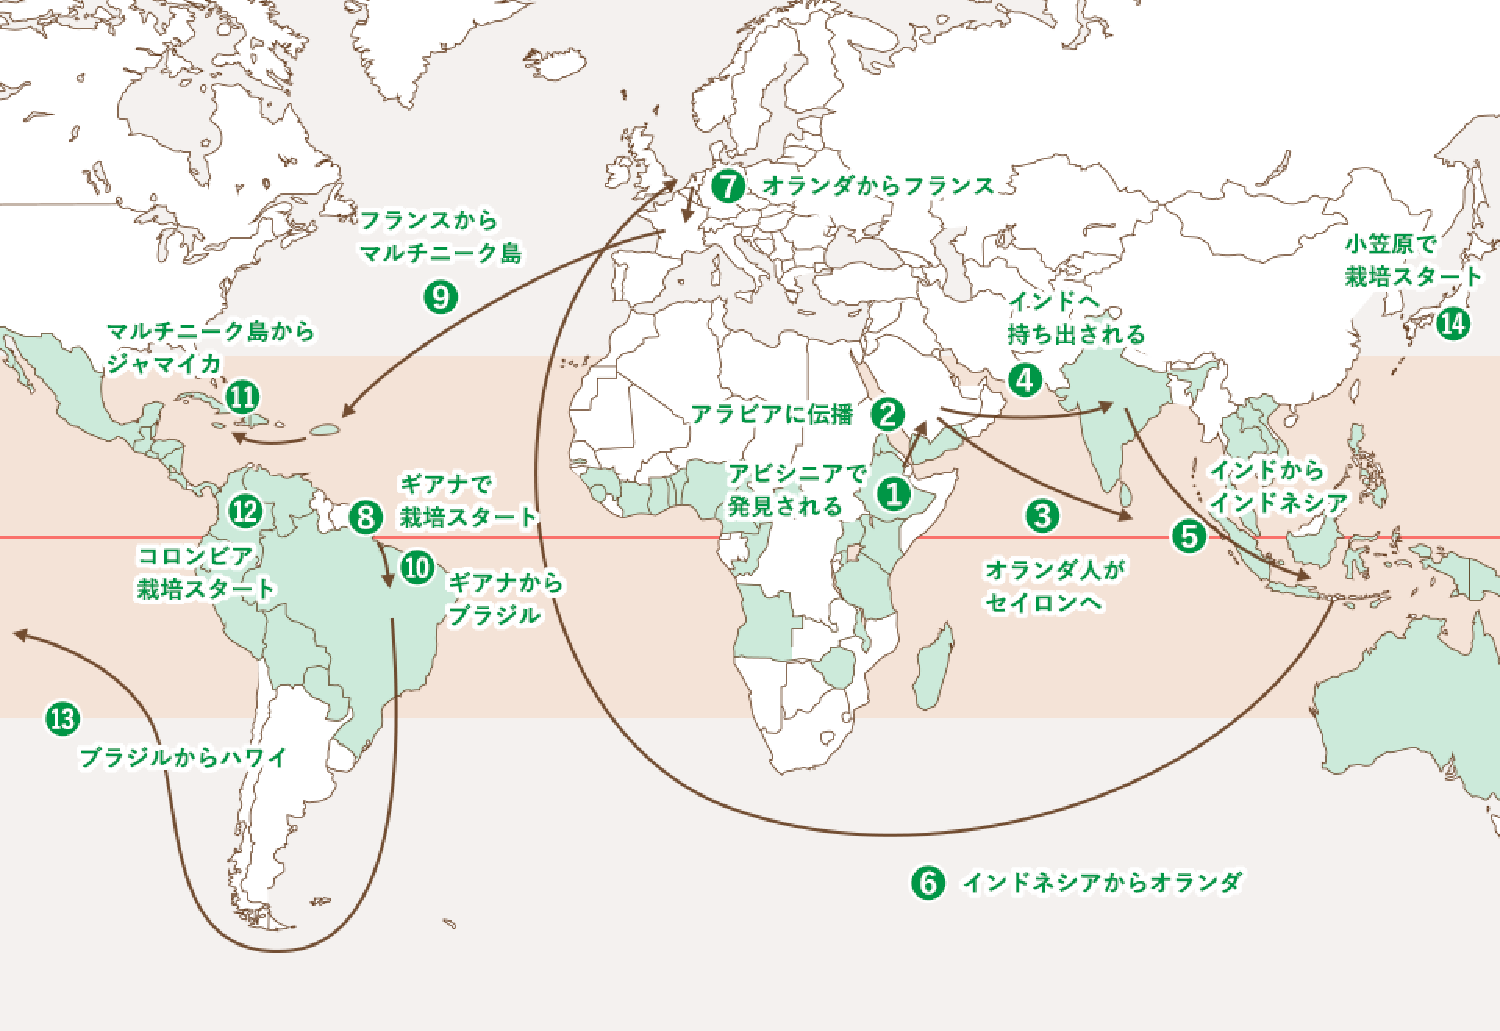
\includegraphics[width=80mm]{figure/map.pdf}
 \end{center}
  \caption{UCCホームページより:コーヒーの軌跡}
  \label{fig:pianosikumu}
\end{figure}


\newpage
\subsection{\large{コーヒーの流行について}}
ここでは,コーヒーの流行を時代別に説明する際に使われる,ウェーブという表現について説明する.
コーヒーはその時代ごとに求められる姿を変え,ファーストウェーブ(第一の波),セカンドウェーブ(第二の波),サードウェーブ(第三の波)へとシフトしていく.
このウェーブという表現は,明確な時間の括りを示すものではないが,流行りの移り変わりとしてコーヒーを語る上で多く用いられる.
\subsubsection{\large{ファーストウェーブ}}
ファーストウェーブ(第一の波)の期間は,1800年代後半\UTF{FF5E}1960年頃と言われている.
この流行はコーヒーの大量消費時代であり,真空保存パックの発明や,インスタントコーヒーが発売された時代でもある.
真空保存パックの発明は,コーヒーの保存期間を劇的に延長し,地方だけでなく大都市でも新鮮なコーヒーが飲めるようになった.
インスタントコーヒーの発明は,コーヒーを楽しむことをより手軽な事とした,第一次・第二次世界大戦においても多くの兵士が愛飲したと言われている.
しかしその反面,この時代のコーヒーは風味がとても乏しく,粗悪品が多く出回る時代でもあった.
\subsubsection{\large{セカンドウェーブ}}
セカンドウェーブ(第二の波)の期間は,1960年頃〜2000年頃と言われている.
ファーストウェーブの際に,一般的かつ手軽な飲み物として普及が進んだコーヒーであったが,普及が進むとともに劣悪な品質が問題化した.
そして,STARBUCKSなどのシアトル発祥のカフェを代表とする,味にフォーカスした流行が起こる,それがセカンドウェーブである.
コーヒーそのものだけでなく,カフェラテなどのエスプレッソドリンクもシアトル系カフェの台頭とともに普及した.
\subsubsection{\large{サードウェーブ}}
サードウェーブ(第三の波)の期間は,2000年頃〜現在も続くと言われている.
セカンドウェーブの際に,品質についての意識が向上したことを皮切りに,高品質かつそのコーヒーの生まれや,農園,淹れ方,加工法などが重視される流行が訪れる事となる.それがサードウェーブコーヒーである.
コーヒーの抽出技術を競う大会や,カップオブエクセレンスと呼ばれるその年のコーヒーで最高品質の物を決める評議会が開催されるなど,一杯の価値にフォーカスされている流行である.
また,昔から日本のカフェで行われてきたハンドドリップは,日本でこそ当たり前の光景だったものの,海外では目新しいものであり,この流行とともに注目を集めていく事となる.
%%%%%%%%%%%%%%%%%%%%%%%%%%%%%%%%%%%%%%%%%%%%%%%%%%

\newpage
\section{\large{抽出方法と抽出器具について}}
本章では,基本的な抽出方法や抽出器具を説明する.

\subsection{\large{抽出方式}}
本節では,抽出の仕組みとも言える抽出方式を説明する.
コーヒーの抽出器具は,それぞれ特有の抽出方式を持っているが,大きく区分したものが以下のものとなる.
\subsubsection{\large{浸漬式}}
浸漬式は,コーヒープレスやコールドブリュー(水出しコーヒー)に代表される抽出方式である.
名前の示す通り,コーヒー豆をお湯や水に浸し,適切な時間漬けておくことで,風味を引き出す.
コーヒーは抽出を過剰に行った場合,雑味やエグ味まで抽出されてしまうため,抽出にかかる時間を適切に管理することが,浸漬式では特に重要である.
比較的長時間の抽出になるため,粗挽きの豆を使用するのが一般的である.特に水出しの場合,お湯に比べ抽出スピードが遅いため,丸一日時間を要する場合もある.
\subsubsection{\large{透過式}}
透過式とは,プアオーバー(ハンドドリップ)やケメックスに代表される抽出方式である.
浸漬式とは異なり,抽出されたコーヒーはフィルターを介し,豆とお湯が分離されサーバーに落とされていく.
日本ではプアオーバーが,喫茶店で長い間提供されていたこともあり,認知度の特に高い抽出方式であるが,海外では比較的目新しい抽出方法である.
\subsubsection{\large{高圧抽出式}}
高圧抽出式は,お湯を浸したコーヒー豆に高い気圧をかけることにより,一気に味を抽出する方式である.
高い圧力をかけるため,風味を濃縮した味わいになりやすい.
\subsubsection{\large{真空濾過式}}
真空濾過式はサイフォンに代表される抽出方式であり,意図的に準真空状態を作り出す方式である.
この方式を採用している器具は少なく,日常で目にする器具はサイフォンがほとんどだが,
同じく真空状態を意図的に利用する器具で,CLOVERと呼ばれる浸漬式と真空バキュームを組み合わせた器具も存在する.

\newpage
\subsection{\large{抽出器具}}
ここでは,数多く存在する抽出器具の一例を説明する.
\subsubsection{\large{コーヒープレス}}
コーヒープレスは,フレンチプレスと呼ばれる器具に,挽いたコーヒー豆とお湯を入れ,時間をかけて抽出を行う器具である.
元はイタリアで
実際の写真を図\ref{fig:press}に示す
紅茶でいうティープレスのように,抽出時間経過後は上からステンレスフィルターを押し下げ,豆と液体を分離することによって,抽出を完了させる.
仕上がりは.多少の粉末感を残すものの,濃厚でまろやかな味わいである.
ステンレスフィルターを使用するため,コーヒーのオイルが吸収されず,コーヒー豆本来の味が楽しめることも利点の一つである.


\begin{figure}[htbp]
 \begin{center}
  \includegraphics[width=80mm]{figure/p4.pdf}
 \end{center}
  \caption{コーヒープレス}
  \label{fig:press}
\end{figure}


\newpage

\subsubsection{\large{プアオーバー}}
プアオーバーは,別名ハンドドリップとも呼ばれている.実際の写真を図\ref{fig:over}に示す
フィルターの上に挽いた豆を置き,お湯を回しかける事によって,下部のグラスサーバーにコーヒーを抽出していく.
フィルターを介しているため,出来上がりは,粉末感は殆どなくクリーンな味わいになりやすい.
また,お湯の注ぐタイミングや蒸らしの時間の掛け方などにより,様々な流派が存在し,淹れた人によって大きく風味が変化する事も特徴の一つである.

\begin{figure}[htbp]
 \begin{center}
  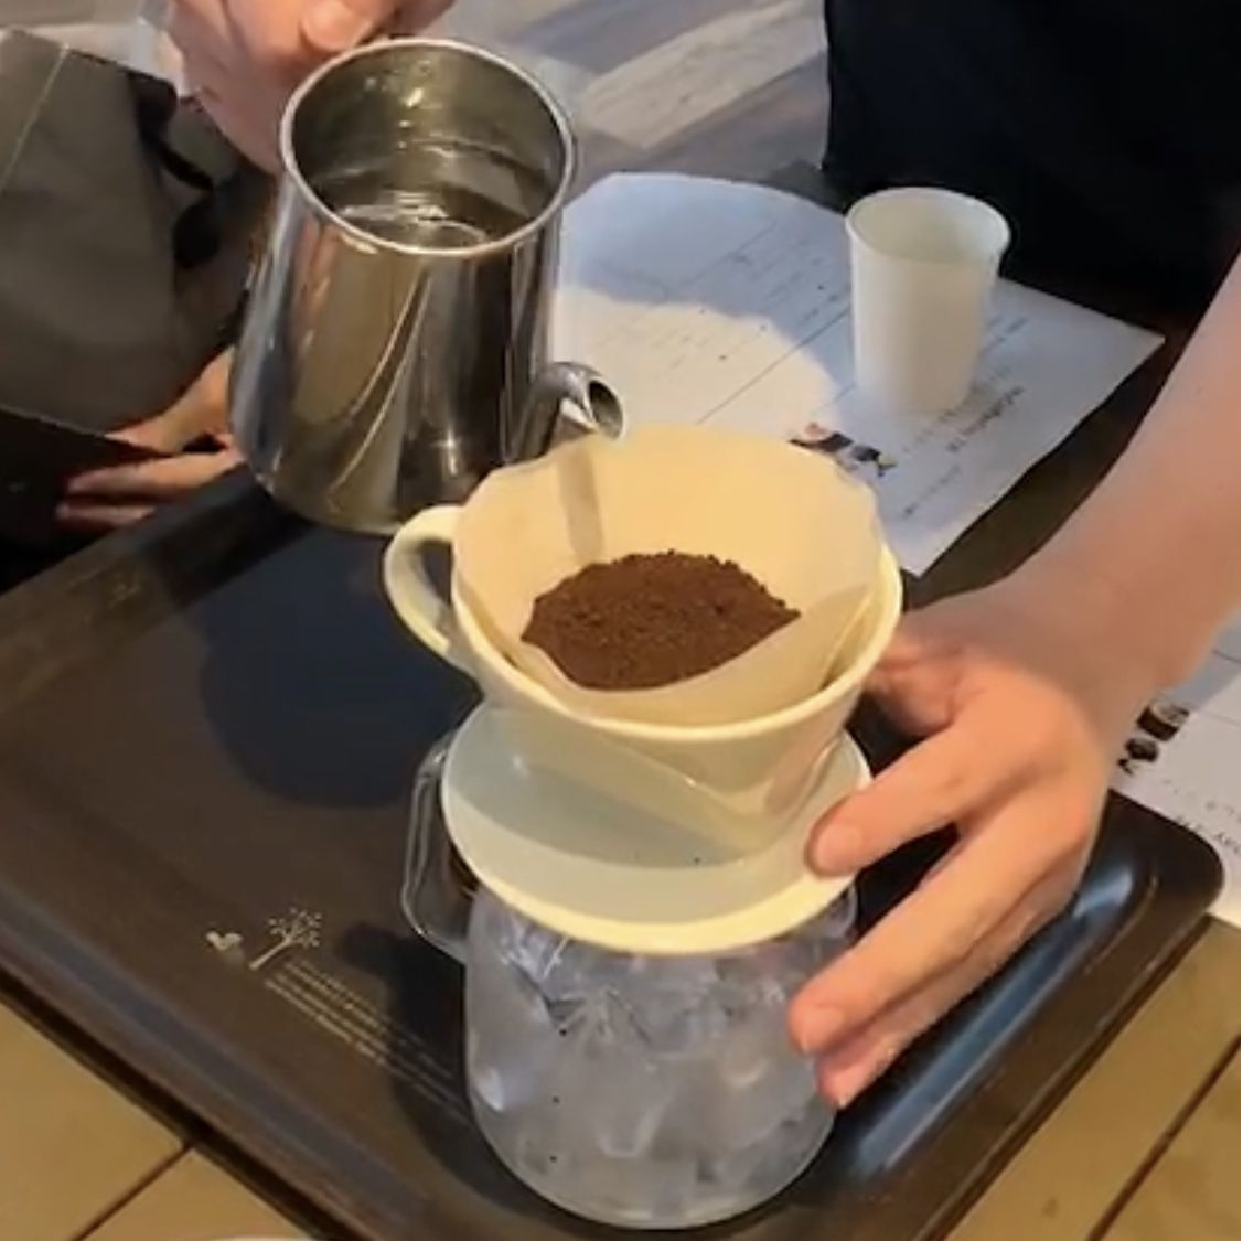
\includegraphics[width=80mm]{figure/set.pdf}
 \end{center}
  \caption{プアオーバー}
  \label{fig:over}
\end{figure}

\newpage

\subsubsection{\large{エスプレッソ}}
エスプレッソは,イタリアを発祥とする飲み方であり,水蒸気やピストンなどで圧力をかけ,短い時間で抽出されたコーヒーのことを指す.
実際の器具の写真を図\ref{fig:esp}に示す
自動式・半自動式・ピストン式など様々なエスプレッソマシンが存在するが,使用者自身でフィルターに豆を押し込み,機械によって気圧をかける半自動式が最も一般的である.
仕上がりは極めて濃厚であり,そのままの状態で飲む以外にも,ミルクを追加しカフェラテ・カプチーノとして提供されることが多い.

\begin{figure}[htbp]
 \begin{center}
  \includegraphics[width=80mm]{figure/e1.pdf}
 \end{center}
  \caption{エスプレッソマシン}
  \label{fig:esp}
\end{figure}

\newpage

\subsubsection{\large{ソロフィルター}}
ソロフィルターは,カフェ等ではあまり提供されないが,コーヒーを初めて淹れる人でも簡単に抽出でき,入門用に最適な器具の一つである.
実際の器具の写真を図\ref{fig:solo}に示す
ステンレスフィルターの上に挽いたコーヒー豆を置いた後,複数の極細の穴があるパーツに規定量のお湯を注ぐだけで,適切な湯量が豆に注がれ続ける.
容量は1杯分のコーヒー豆しか入らないため,大人数分のコーヒーを抽出するには不向きだが,粉末感の殆どない高品質なコーヒーを手軽に味わえるため,
コーヒーを学び始めの人や,朝の忙しい時間でも簡単に抽出することができる.

\begin{figure}[htbp]
 \begin{center}
  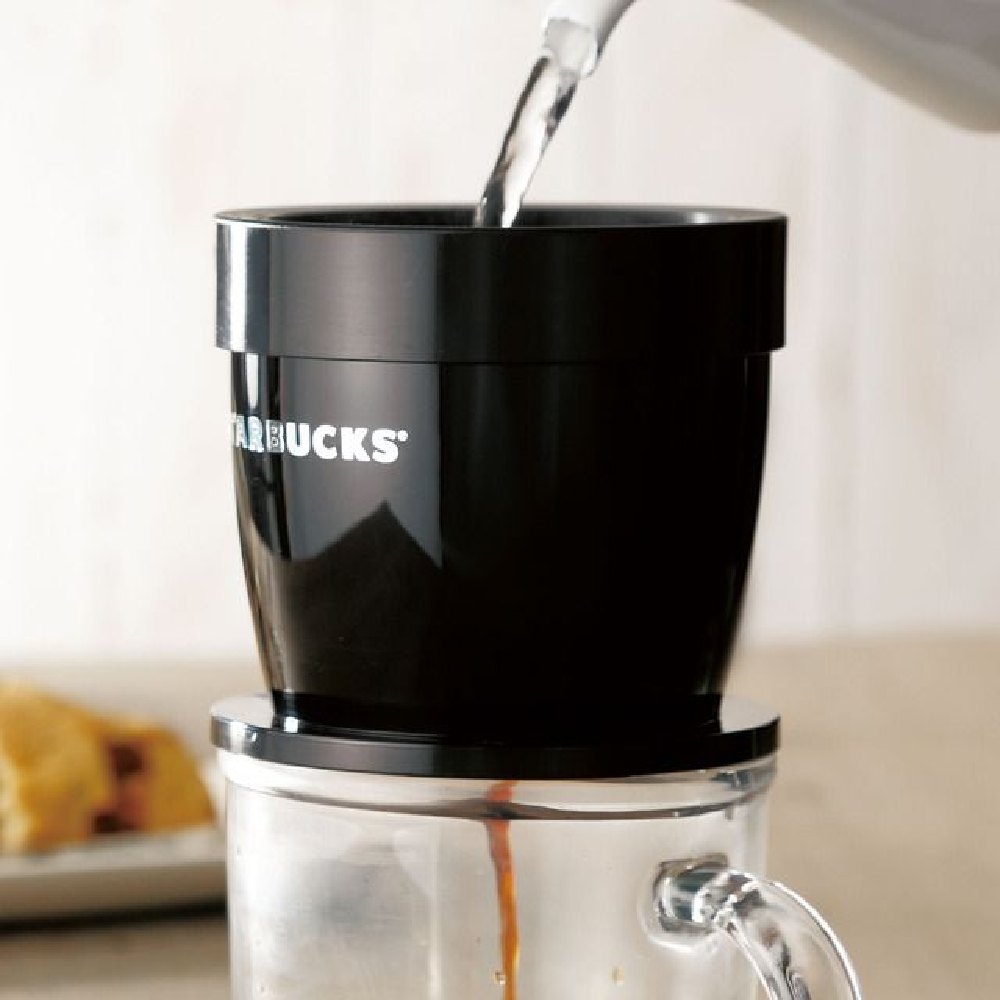
\includegraphics[width=80mm]{figure/gazou6.pdf}
 \end{center}
  \caption{ソロフィルター}
  \label{fig:solo}
\end{figure}

\newpage


\subsubsection{\large{サイフォン}}
サイフォンは,科学の実験器具のような形状をした抽出器具であり,数ある抽出器具の中でも特に見栄えの良い器具として,注目を集めている.
実際の器具の写真を図\ref{fig:siphon}に示す
お湯を熱したことによる蒸気圧を使用し,真空に近い状態を作り出すことで,コーヒーが器具の内部を上下し,フィルターを通して濾過される.日本の喫茶店でも多く取り入れられていたため,馴染みの深い抽出器具でもある.
従来は加熱にアルコールランプを使用していたが,最近では電気式が主流となっている.

\begin{figure}[htbp]
 \begin{center}
  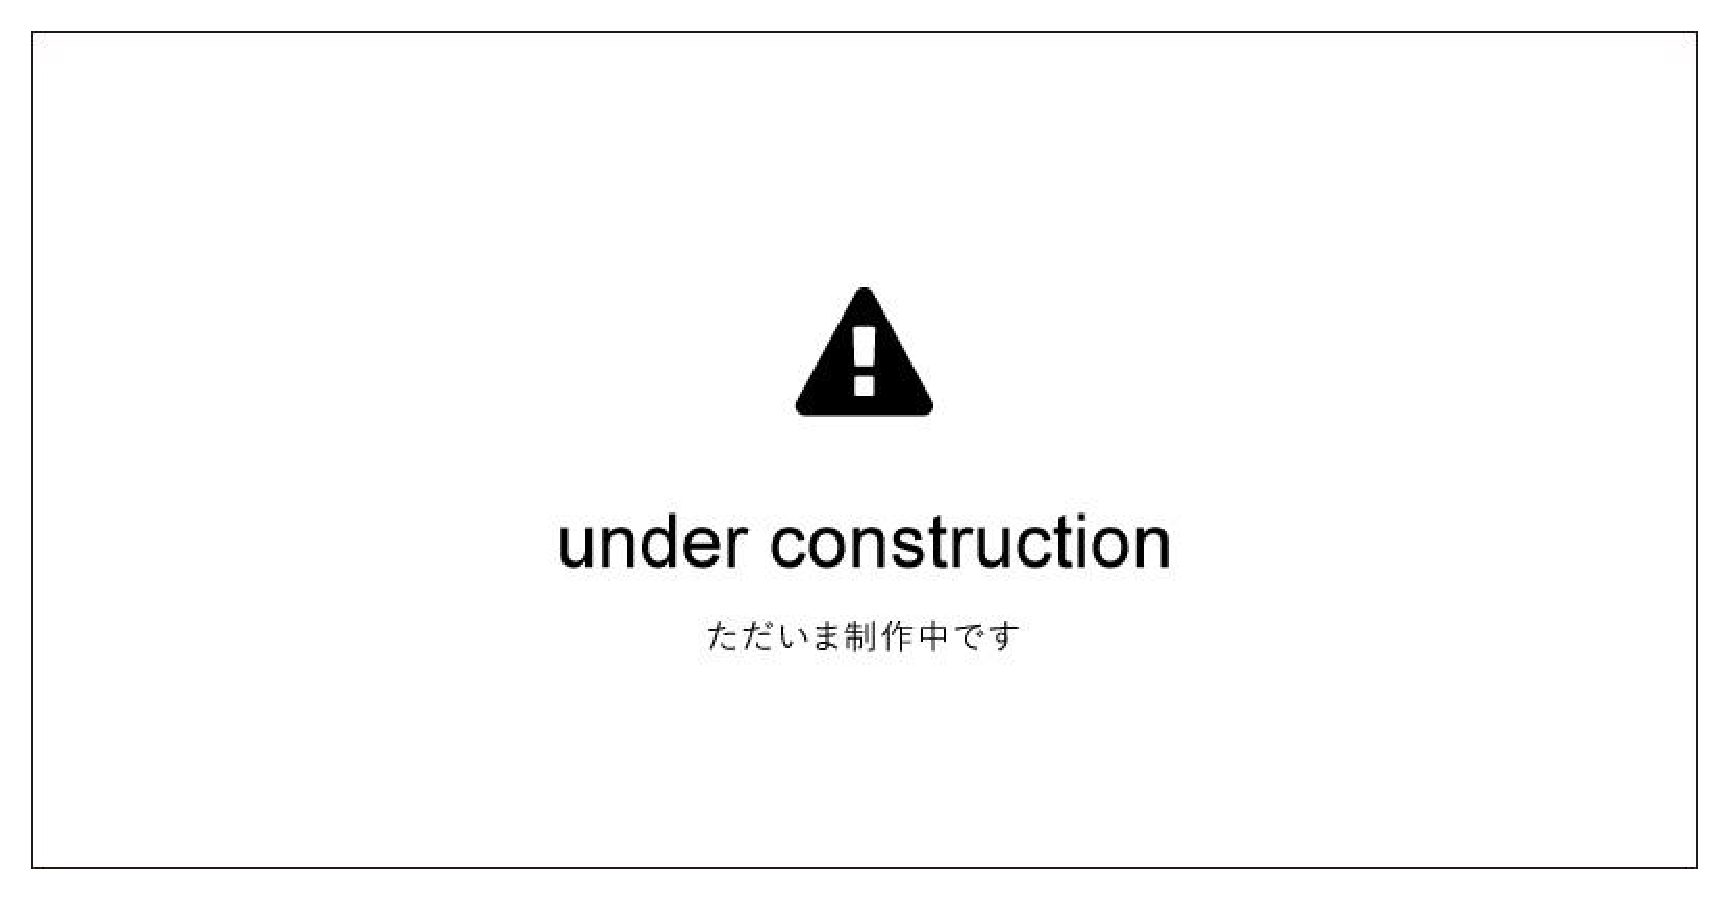
\includegraphics[width=80mm]{figure/seisakutyuu.pdf}
 \end{center}
  \caption{サイフォン}
  \label{fig:siphon}
\end{figure}

\newpage

\subsubsection{\large{クレバードリッパー}}
クレバードリッパーは,近年新たに提案された浸漬式と透過式を合わせた抽出器具である.
実際の器具の写真を図\ref{fig:cl}に示す
コーヒープレスと同様に,コーヒー豆をお湯に浸し適切な時間をおいた後,ペーパーフィルターを通し,豆とお湯を分離する抽出方法をとる.
味わいは,浸漬式のマイルドさと,透過式のスッキリさを併せ持っている.一度に多くのコーヒーを抽出できるほか,プアオーバーのような複雑な工程を踏まないため,比較的簡単に抽出を行うことができる.

\begin{figure}[htbp]
 \begin{center}
  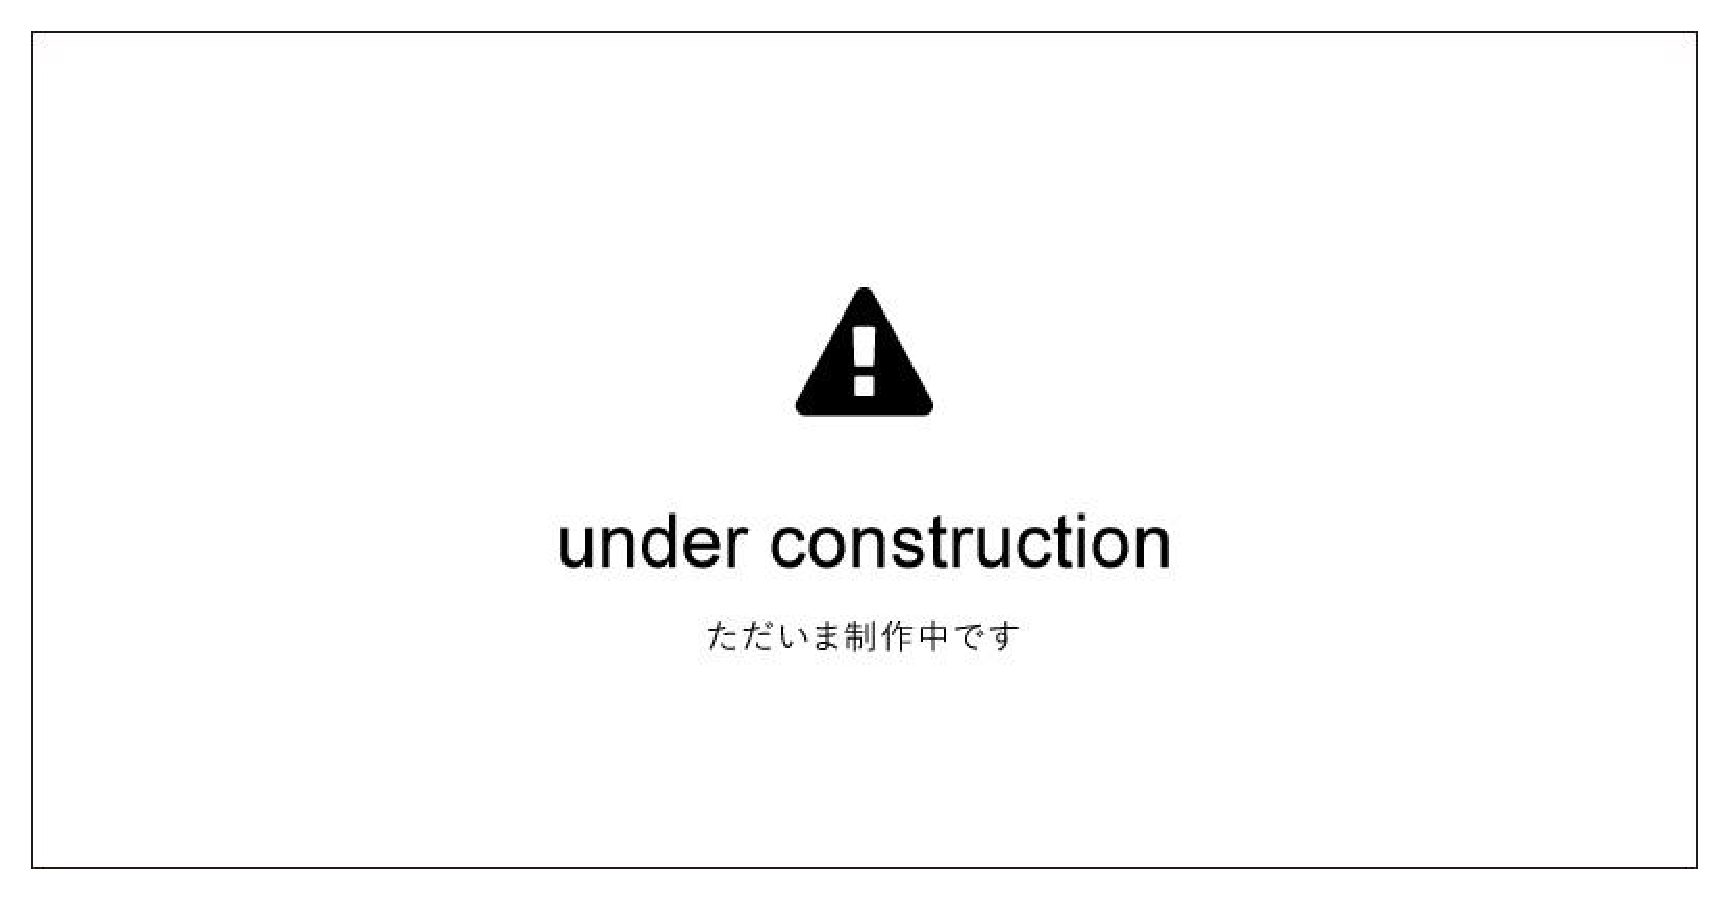
\includegraphics[width=80mm]{figure/seisakutyuu.pdf}
 \end{center}
  \caption{クレバードリッパー}
  \label{fig:cl}
\end{figure}

\newpage

\subsubsection{\large{エアロプレス}}
実際の器具の写真を図\ref{fig:aero}に示す
エアロプレスは,その名の通り空気圧を使用した抽出器具である.開発されたのは2005年であり,数多くの抽出器具の中でも特に直近に提案された器具である.
注射器のような形状をしており,利用者自身が器具を押し込むことによって,空気圧を調整し抽出を行う.
抽出時間が短いこと,味わいが濃厚であることが特徴である.
2005年という直近の開発でありながら,様々なカフェで提供されている他,エアロプレスに特化した,抽出技術を競う大会が開催されたりと,シェアを順調に伸ばしている.

\begin{figure}[htbp]
 \begin{center}
  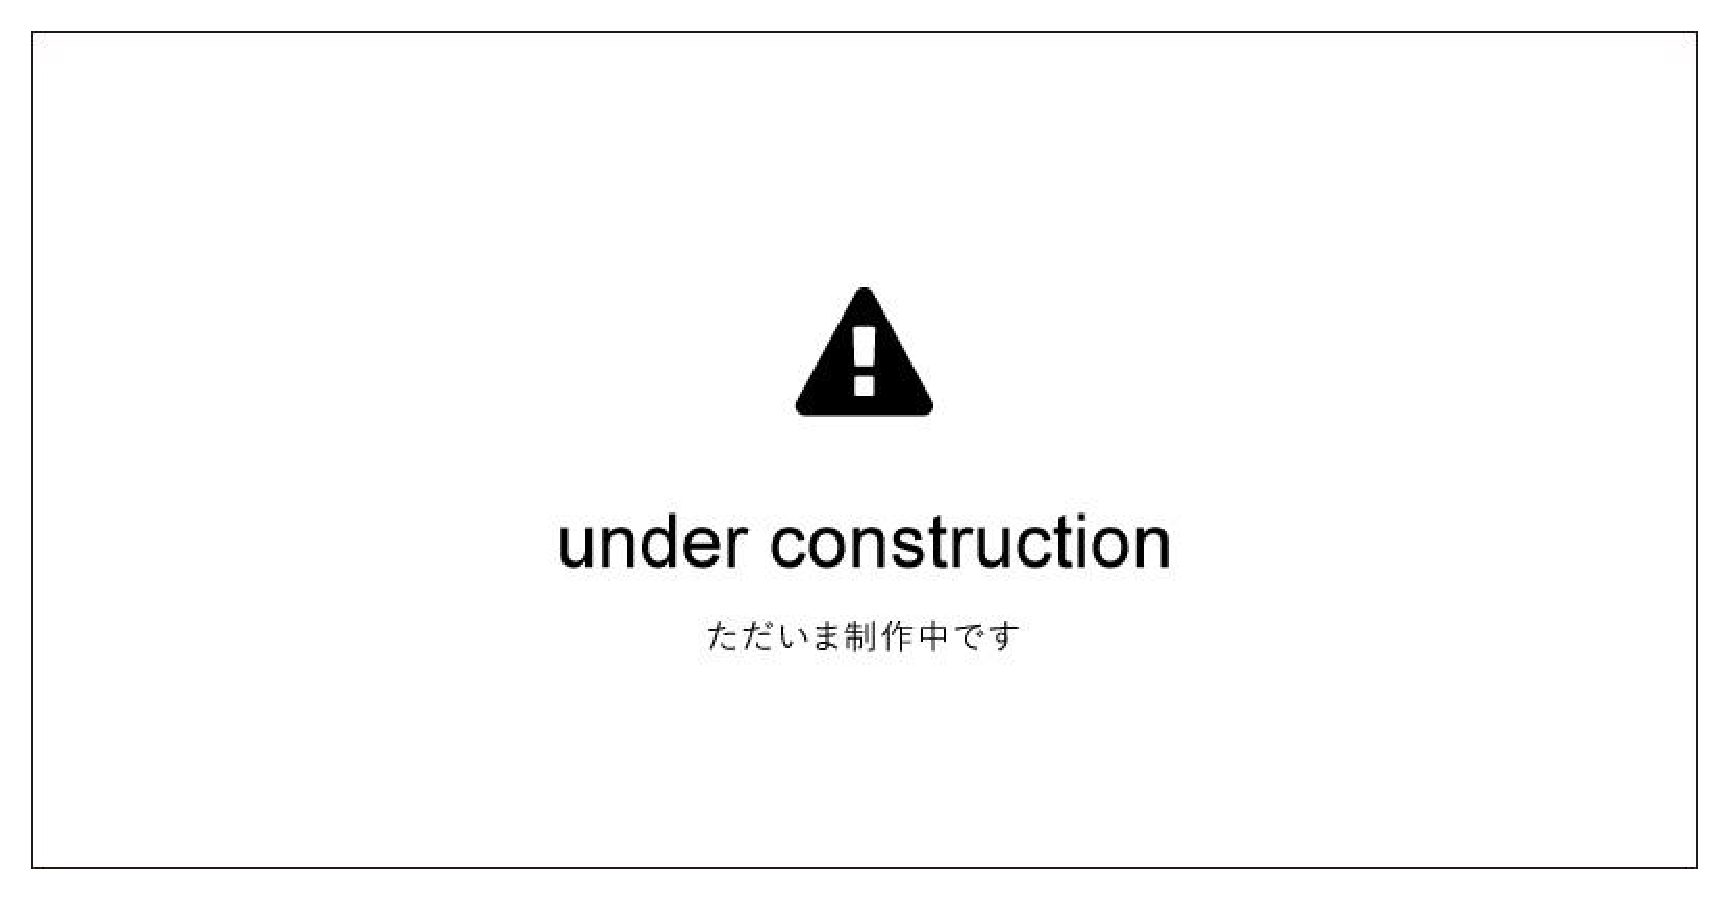
\includegraphics[width=80mm]{figure/seisakutyuu.pdf}
 \end{center}
  \caption{エアロプレス}
  \label{fig:aero}
\end{figure}


%%%%%%%%%%%%%%%%%%%%%%%%%%%%%%%%%%%%%%%%%%%%%%%%%%

\newpage
\section{\large{コーヒー抽出の学習方法}}
本章では,コーヒー抽出の基本的な学習方法を説明する.

\subsection{\large{抽出の基本的な学習方法}}
コーヒー抽出の学習方法は,他の学問と同様に様々な学習スタイルが存在する.
近年では,多くの個人経営カフェや,チェーン店においてもコーヒーセミナーという形で,実践を伴った学習ができる.
また個人学習においては,抽出に関することに主題を置いた書籍が多数出版されている他,インターネット上で抽出レシピやコツなどを簡単に閲覧することができる.
\subsubsection{\large{コーヒーの学習が可能なWebサイトついて}}
インターネット上のWebサイトでは,コーヒーの基本知識から,実際の抽出方法に至るまで多くの情報が閲覧できる.
個人で運営されているWebサイトだけでなく,コーヒー業界の大手であるUCCや,STARBUCKS,TULLY'Sなどの企業も自社ページで,器具ごとの抽出手順や実際の抽出動画を公開している.

\subsubsection{\large{既存の音声認識可能なWebレシピについて}}
既存の音声認識可能なWebレシピで特に有名なものとして,クックパッドが挙げられる.このWebレシピは,料理レシピの閲覧・投稿が可能であり,調理手順をステップごとに確認することができる.元々は音声認識は実装されていなかったが,Amazonが発売している,スマートスピーカー「Amazon Echo」のクックパッドスキルを使用することで,音声認識が使用できる.機能は主にレシピの検索や読み上げであり,画面ではなく音声を聞きながらの調理をすることになる.
スマートフォンアプリで使用できるものとしては,macaroniというWebレシピが存在する.こちらは,調理動画を閲覧する際に音声認識が可能であり,「サイセイ」,「マキモドシ」などの発音で,動画の再生をコントロールできる.
%%%%%%%%%%%%%%%%%%%%%%%%%%%%%%%%%%%%%%%%%%%%%%%%%%


%%%%%%%%%%%%%%%%%%%%%%%%%%%%%%%%%%%%%%%%%%%%%%%%%%

\newpage
\section{\large{プログラミング言語と音声認識ついて}}
本章では,システムを制作する上で利用するプログラミング言語と音声認識について説明する.
\subsection{\large{HTML・CSSとは}}
HTML(Hyper Text Markup Language)とは,プログラミング言語の1つである.主にWebページを作成する際に使用される言語である,
単なる文字の集まりである文章に,見出し・ボタン・リストなどの役割を指定し,コンピュータに認識させることができる.
現存するほとんどのWebページがHTMLによって構造を作られている.

CSS(Cascading Style Sheets)とは,HTMLに記載された役割を持つ文章に対し,サイズ指定を行うことや,文字色の変更,配置を調整することができる言語である.
HTML単体の記述では,単調な文章表記やレイアウトになってしまうため,多くのWebサイトでCSSを用いたデザイン調整が行われている.
使用方法は,HTMLファイルから別のCSSファイルを読み込むというだけでなく,HTMLファイル中に直接CSSを書くこともできるなど,用途に合わせた柔軟な記述ができるようになっている.

\subsection{\large{音声認識とは}}
音声認識とは,人間が発する声をコンピュータ上で解析を行い,テキストとして認識する技術である.
\subsubsection{\large{音声認識の仕組み}}
音声認識の仕組みは利用するサービスによって異なるほか,その時代によっても音声認識の方法論が移り変わっている.
河原(2018)の,音声認識の方法論の変遷を表として,表ref{tb:onsei}に示す.
この表1を見ると現在の音声認識の方法論は4.5世代にあたり,ニューラルネットワークの利用が主流になっていることがわかる.
ニューラルネットワークはいわば機械学習の類であり,それらを応用することで音声認識を成し遂げている.
実際に,Google社の手がける音声認識サービス「Google Cloud Speech API」においてもニューラルネットワークモデルが利用されていることが明記されている\cite{Railshon1}.

\begin{table}[h]
\begin{center}
\caption{音声認識の方法論の変遷(河原,2018)}
\begin{tabular}{| l | c | c | c |}  \hline
第1世代  & 1950\UTF{FF5E}1960年代 & ヒューリスティック                 \\ \hline
第2世代  & 1960\UTF{FF5E}1980年代 & テンプレート (DP マッチング, オートマトン) \\ \hline
第3世代  & 1980\UTF{FF5E}1990年代 & 統計モデル (GMM-HMM, N-gram)   \\ \hline
3.5世代 & 1990\UTF{FF5E}2000年代 & 統計モデルの識別学習                \\ \hline
第4世代  & 2010年代      & ニューラルネット (DNN-HMM, RNN)   \\ \hline
4.5世代 & 2015年\UTF{FF5E}      & ニューラルネットによる End-to-End    \\ \hline
\end{tabular}
\label{tb:onsei}
\end{center}
\end{table}


\subsubsection{\large{WebSpeechAPI}}
WebSpeechAPIとは,JavaScriptAPIの1つである.
JavaScriptとWebブラウザのみで,音声の合成や音声認識を可能にする.
音声の合成は入力した文字を機械側に発音させる機能であり,音声認識は音声をテキストとして入力する機能である,
本Webアプリケーションの音声認識はこのWebSpeechAPIを使用している.
\subsubsection{\large{音声認識を可能にするJavaScriptについて}}
音声認識を可能にするJavaScriptは,宗定(2014)の記事を元に作成した「seramic.js」\cite{Railshon2},
ページ間の移動を制御する「page.js」,「nylon.js」の3つのファイルによって実装している.
「seramic.js」ファイルはWebSpeechAPIを用い,継続的に音声を聞き取り続けるためのプログラムである.
「次へ」,「戻る」の発音がされた場合,「page.js」,「nylon.js」を呼び出し,ページの移動が行われる.
フローチャートを図\ref{fig:huro}に示す

\begin{figure}[htbp]
 \begin{center}
  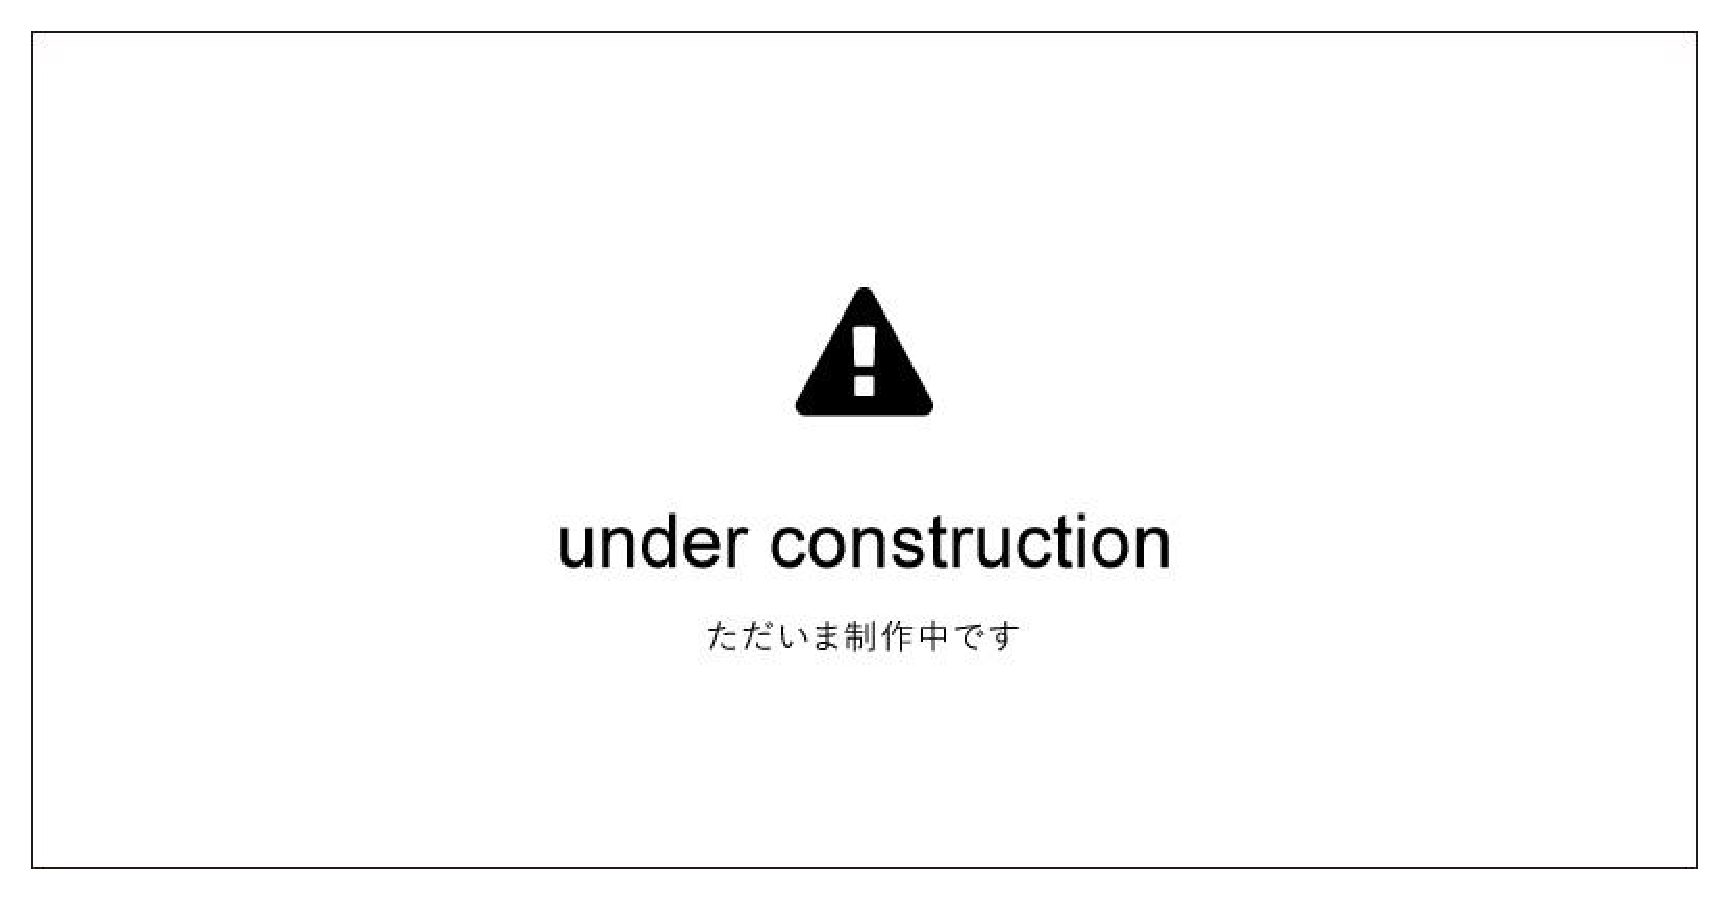
\includegraphics[width=80mm]{figure/seisakutyuu.pdf}
 \end{center}
  \caption{音声認識フローチャート}
  \label{fig:huro}
\end{figure}


\subsubsection{\large{音声認識によるページ移動}}

%%%%%%%%%%%%%%%%%%%%%%%%%%%%%%%%%%%%%%%%%%%%%%%%%%

\newpage
\section{\large{本研究で開発するWebレシピの概要}}
本章では,実際に制作するシステムについて説明する.
\subsection{\large{コンセプトとページ構成について}}
コーヒーの抽出は目的に合わせ抽出器具を使い分けるため,それぞれの特徴を踏まえた上で器具の選定を行うことが重要である.
そのため,本研究で開発したWebレシピのページは,「抽出器具選択画面」,「レシピ閲覧画面」の二段階で構成している.
抽出器具選択画面において,利用者はそれぞれの器具の特徴や風味の違いを理解し,レシピ閲覧画面で実際の抽出をサポートする.
本レシピアプリのページ構成を図\ref{fig:kousei}に示す.


\begin{figure}[htbp]
 \begin{center}
  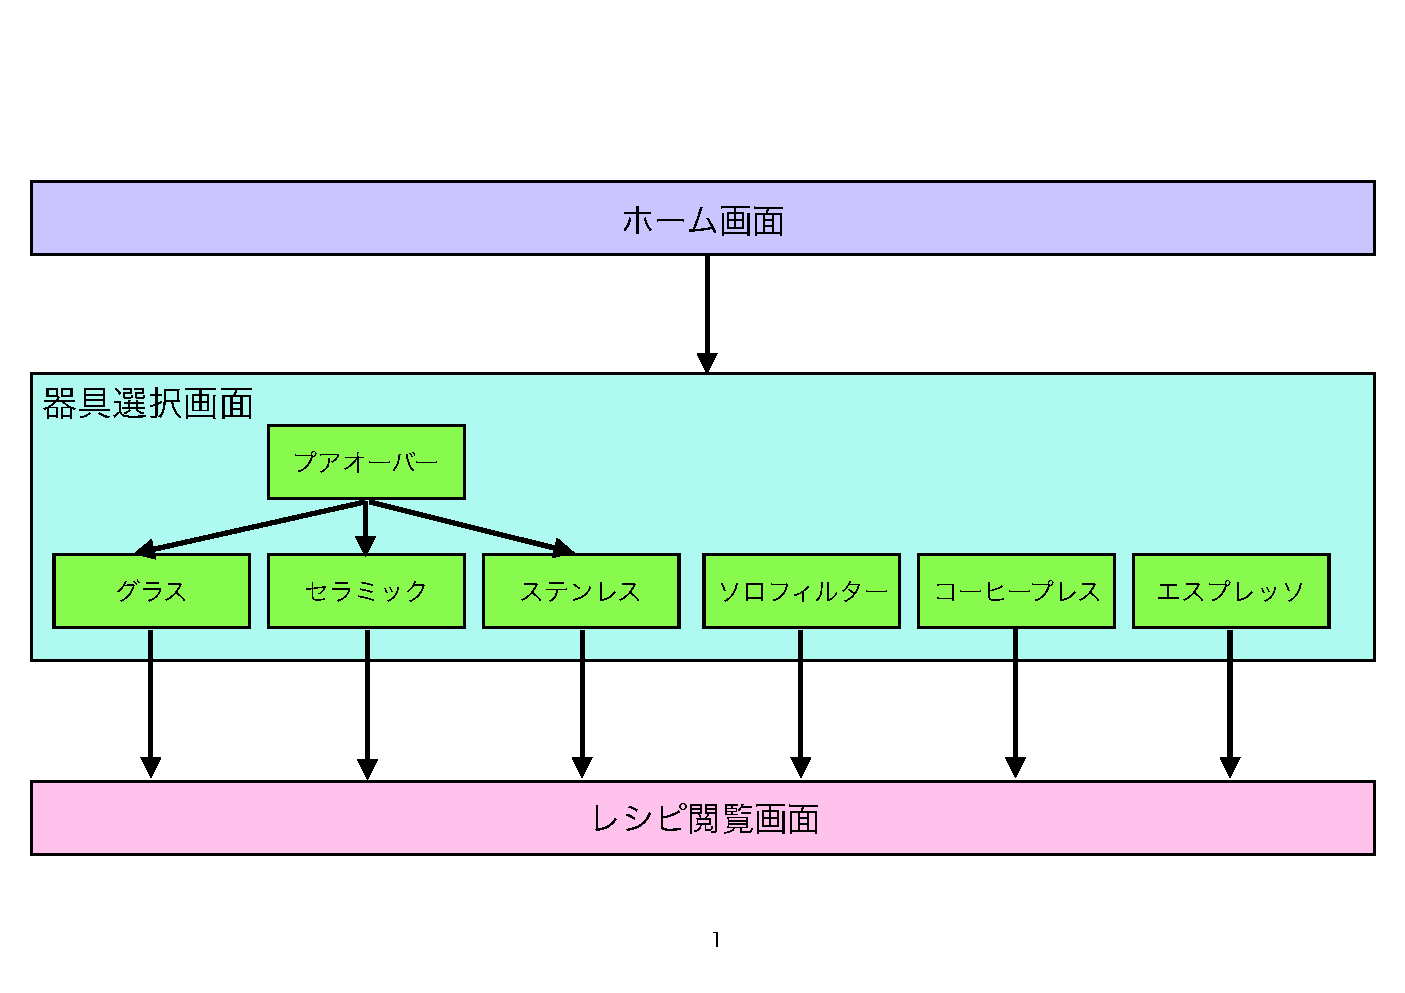
\includegraphics[width=100mm]{figure/kousei.pdf}
 \end{center}
  \caption{ページ構成}
  \label{fig:kousei}
\end{figure}




\subsection{\large{実装機能}}
本研究で実装する機能は,「コーヒーの専門性の高いWebレシピの機能」と「音声認識」である.
「コーヒーの専門性の高いWebレシピの機能」は,コーヒーの抽出器具ごとの情報や,その組み立て方および抽出手順である.
前節にて述べたとおり,抽出をする際に使用する器具の特徴をあらかじめ理解していることはとても重要である.
抽出手順においても器具ごとに異なるため,そのステップごとに個別のページを用意し,順に解説を行う.

「音声認識」は,抽出ステップ間の移動を行う際に使用する.
実際の抽出中は両手が塞がることが多く,ページ移動のボタンを押せないことが予期されるため,ボタンの他に音声認識でもページを移動できるようにする.

\newpage


\subsubsection{\large{抽出器具選択画面}}
「抽出器具選択画面」では,レシピを閲覧する抽出器具を選択する.
実際の抽出器具選択画面を図\ref{fig:kigusentaku}に示す.

この画面では,抽出方式の異なる3つの代表的な抽出器具と,ソロフィルターを含めた4種類を選択できる.
プアオーバー(透過式),コーヒープレス(浸漬式),エスプレッソ(高圧抽出式)は,日本で特に馴染みの深いコーヒーの抽出方法であり,様々なカフェで提供されていることから選択した.
ソロフィルター(より手軽な入門向け)は,カフェ等ではあまり提供されないが,コーヒーを初めて淹れる人でも簡単に抽出でき,入門用の器具の一つとして選定した.

「レシピを見る」を選択することで,「レシピ閲覧画面」へと移動する.

「レシピ閲覧画面」では,実際に器具ごとのコーヒー抽出レシピを閲覧できる.

\begin{figure}[htbp]
 \begin{center}
  \includegraphics[width=130mm]{figure/soturon2.pdf}
 \end{center}
  \caption{抽出器具選択画面}
  \label{fig:kigusentaku}
\end{figure}

\newpage

\subsubsection{\large{レシピ閲覧画面}}
「レシピ閲覧画面」では,実際に器具ごとのコーヒー抽出レシピを閲覧できる.
実際のレシピ閲覧画面を図\ref{fig:recipieturan}に示す.

ページは抽出ステップごとに分割している.
1つのステップ毎に,個別の画像と説明文を表示し,記載されている指示に従うことで,抽出を行うことができる.
ステップ間は,画面上部のボタンを押すことで移動が可能であるほか,音声認識も実装している.
画面下部の「音声認識を開始する」ボタンを押すことにより,音声認識処理が開始し,「次へ」・「戻る」の発音で,ステップ間の移動が可能である.

\begin{figure}[htbp]
 \begin{center}
  \includegraphics[width=130mm]{figure/soturon1.pdf}
 \end{center}
  \caption{レシピ閲覧画面}
  \label{fig:recipieturan}
\end{figure}

\newpage.


%%%%%%%%%%%%%%%%%%%%%%%%%%%%%%%%%%%%%%%%%%%%%%%%%%



%%%%%%%%%%%%%%%%%%%%%%%%%%%%%%%%%%%%%%%%%%%%%%%%%%

\newpage
\section{\large{結言}}
%音楽は趣味や仕事の面で多くの人が関わり,古代から現代まで長く続いている文化である.職種としてのみならず,趣味としても多くの人にあげられる音楽は世界共通の言語なのである.
コーヒーは,1章にて述べた通り,長い年月をかけて愛され,世界の人々を魅了してきた.
また,その生産に当たっても,農家・バイヤー・焙煎士・加工者など多くの人々の手に渡りながら世界を巡り,最終的に消費者の元に訪れる.
そのような長い過程を経たとしても,最終的には抽出次第で味は如何様にも変化する.
難しいと感じる人も多いだろうが,そこがコーヒーの魅力でもあり,人々を惹きつける要因の1つだろう.

%特にピアノは歌やその他の楽器との相性が良いことから楽器としては最も多くの人に関与するものであり,その分奏者人口も多いことが挙げられる.
%ピアノを学ぶ上で楽譜は必要不可欠な要素であり,今後も多くの人々が楽譜と関わることになる.しかし,ピアノの楽譜は初心者にとって難しく,挫折の要因の1つとして挙げられる.
しかし,抽出手順や器具ごとの特徴の違いなどから学習の難易度が高くなり,コーヒーを淹れることの敷居も高くなっている実情は,その楽しみを阻害するだけでなく,新たなコーヒーの楽しみ方を模索する機会を失ってしまっている問題点がある.
また実際の抽出中は両手が塞がってしまうのに対し,現存のWebレシピでは音声認識を実装していない,もしくはコーヒーの専門性が低いという問題点があった.
%そこで本研究では,ピアノ指導者が各音符に手書きで音階を書き込む際,指導者にとって時間的コストがかかっている現状を問題点とし,その対策として実際に音階表示補助システムを開発し,ピアノ指導者に評価してもらうことを目的とした.
そこで本研究では,様々な抽出器具のレシピが閲覧可能であり,音声認識によってページ移行が可能なWebレシピを開発し,問題点の解決に取り組んだ.
%実際にOpenCVとPythonを利用し,音階を認識するシステムを制作した.実際に音階を表示し,ピアノ指導者の評価を得た.本システムを導入するかの差があるとはいえ,時間的コスト削減の面で本システムは大きく貢献できることがわかった.
%また,今後の展望としては音階の表示のみならず,音階表示のパターンを変化,音階表示以外の視覚サポート,音によるサポート等ができるとより良いシステムになる.
今回の開発で,気軽にコーヒー抽出を行うことのサポートとして第一歩を踏み出せたと考えている.
今後このような,抽出アシストツールがより普及し,コーヒーを抽出できるようになることを期待している.

%%%%%%%%%%%%%%%%%%%%%%%%%%%%%%%%%%%%%%%%%%%%%%%%%%

\newpage
\section*{謝辞}
本研究の遂行及び本論文の作成にあたり,須田研究室の仲間に深く感謝の意を表します.そして,何よりも本論文の作成にあたり,多大なる御指導及び御助言を頂きました須田宇宙准教授に深く感謝の意を表します.

%%%%%%%%%%%%%%%%%%%%%%%%%%%%%%%%%%%%%%%%%%%%%%%%%%
%参考文献
\newpage
\section{\large{参考文献}}\label{参考文献}
\begin{thebibliography}{9}
%\bibitem{kawahara}名前, ``書籍名'', 出版, Vol71, No11, 年, pp197-203
\bibitem{Railshon1} 
google , ``Cloud Speech-to-Text'', \url{https://cloud.google.com/speech-to-text/?hl=ja}\\
\bibitem{Railshon2} 
宗定 洋平, ``[HTML5] Web Speech APIに入門', \url{https://www.yoheim.net/blog.php?q=20140701}\\
\bibitem{Railshon3} 
OpenCV team,``OpenCV'',\url{https://opencv.org/}\\
\bibitem{Railshon4} 
Python Software Foundation, ``Python'', \url{https://www.python.org/}\\
\bibitem{Railshon5} 
神奈川工科大学 情報学部 情報工学科 信号処理応用研究室 , ``標準画像/サンプルデータ'', \url{http://www.ess.ic.kanagawa-it.ac.jp/app_images_j.html#image_dl}\\

\bibitem{Railshon6} 
paulrosen , ``abcjsデモページ'', \url{https://abcjs.net/abcjs-editor.html}\\

\bibitem{Railshon7} 
KoheiShitaune,``TrainingAssistant'',\url{https://github.com/shkh/TrainingAssistant}\\

\bibitem{Railshon8} 
教育芸術社 市川都志春 編著,``こどものバイエル第1集'',2004年10月30日初版発行,2018年3月第34版発行,pp5\\

\bibitem{Railshon9} 
株式会社ドレミ楽譜出版社 橋本晃一 編著,``中級レベルで弾けるクラシック名曲ピアノ曲集'',1994年1月初版発行,2007年2月20日第7版発行,pp26-27\

\end{thebibliography}
%%%%%%%%%%%%%%%%%%%%%%%%%%%%%%%%%%%%%%%%%%%%%%%%%%
%付録
\newpage
\newgeometry{left=2cm,bottom=2cm}
\appendix
\section{作成したプログラム}

\section*{Square.py}
\label{Square.py}
\listinginput{1}{program/Square.py}
\newpage

\section*{Circle.py}
\label{Circle.py}
\listinginput{1}{program/Circle.py}
\newpage

\section*{Decision.rb}
\label{Decision.rb}
\listinginput{1}{program/Decision.rb}
\newpage

\section*{Line.py}
\label{Line.py}
\listinginput{1}{program/Line.py}
\newpage

\section*{index.py}
\label{index.py}
\listinginput{1}{program/index.py}
\restoregeometry

\end{document}